\chapter{Basic calculus and trigonometry}

\begin{abstract}
    Here, I assume you already have a knowledge of trigonometry. This chapter is built to reinforce that and unify trigonometry with calculus. I still try to keep the same theme throughout; having the geometrical interpretation vivid. This chapter will explore
    \begin{enumerate}[noitemsep]
        \item The physical interpretation of derivatives and integrals of trigonometric function
        \item The relationship between trignometric functions and exponentials
        \item Newton's law in other coordinates
    \end{enumerate}
    We'll extensively use trigonometry in \cref{sec:significanceofcalculus}. Also, this chapter might seem a bit dry because there are no examples that I can give yet without learning about trigonometry first.
\end{abstract}

\section{Basic trigonometric identities}

Here I assume that the reader is already familiar with the basic trigonometric identities and their physical interpretation; therefore, I shall just list them out.
\begin{table}[ht]
    \centering
    \begin{tabular}{l | l | l}
        Function & Domain & Range \\
        \hline
        $\sin(\theta)$ & $(-\infty, \infty)$ & $[-1, 1]$ \\
        $\cos(\theta)$ & $(-\infty, \infty)$ & $[-1, 1]$ \\
        $\tan(\theta)$ & $(-\infty, \infty) - \{\theta | \cos\theta = 0\}$ & $(-\infty, \infty)$ \\
        $\csc(\theta)$ & $(-\infty, \infty) - \{\theta | \sin\theta = 0\}$ & $(-\infty, 1] \cup [1, \infty)$ \\
        $\sec(\theta)$ & $(-\infty, \infty) - \{\theta | \cos\theta = 0\}$ & $(-\infty, 1] \cup [1, \infty)$ \\
        $\cot(\theta)$ & $(-\infty, \infty) - \{\theta | \sin\theta = 0\}$ & $(-\infty, \infty)$ \\
        $\arcsin(\theta)$ & $[-1, 1]$ & $[-\flatfrac{\cpi}{2}, \flatfrac{\cpi}{2}]$ \\
        $\arccos(\theta)$ & $[-1, 1]$ & $[0, \cpi]$ \\
        $\arctan(\theta)$ & $(-\infty, \infty)$ & $(-\flatfrac{\cpi}{2}, \flatfrac{\cpi}{2})$ \\
        $\arccot(\theta)$ & $(-\infty, \infty)$ & $(0, \cpi)$ \\
        $\arcsec(\theta)$ & $(-\infty, 1] \cup [-1, \infty)$ & $[0, \flatfrac{\cpi}{2}) \cup (\flatfrac{\cpi}{2}, \cpi]$ \\
        $\arccsc(\theta)$ & $(-\infty, 1] \cup [-1, \infty)$ & $[-\flatfrac{\cpi}{2}, 0) \cup (0, \flatfrac{\cpi}{2}]$
    \end{tabular}
    \caption{Table of domains and range of trigonometric functions}
\end{table}

Pythagoras's identities:
\begin{equation*}
    \sin[2](\theta) + \cos[2](\theta) = 1,\quad 1 + \tan[2](\theta) = \sec[2](\theta), \quad 1 + \cot[2](\theta) = \csc[2](\theta).
\end{equation*}
Angles addition:
\begin{gather*}
    \sin(A + B) = \sin A\cos B + \sin B\cos A, \\
    \sin(A - B) = \sin A\cos B - \sin B\cos A, \\
    \cos(A + B) = \cos A\cos B - \sin A\sin B, \\
    \cos(A - B) = \cos A\cos B + \sin A\sin B. 
\end{gather*}
Double angles formulas:
\begin{gather*}
    \sin(2\theta) = 2\sin\theta\cos\theta, \\
    \cos(2\theta) = \cos[2](\theta) - \sin[2](\theta) = 1 - 2\sin[2](\theta) = 2\cos[2](\theta) - 1, \\
    \tan(2\theta) = \frac{2\tan\theta}{1 - \tan[2](\theta)}.
\end{gather*}
Triple angles formulas:
\begin{gather*}
    \sin(3\theta) = 3\sin(\theta) - 4\sin[3](\theta), \\
    \cos(3\theta) = 4\cos[3](\theta) - 3\cos(\theta).
\end{gather*}
Half angles formulas:
\begin{gather*}
    \sin(\frac{\theta}{2}) = \sqrt{\frac{1 - \cos\theta}{2}}, \\
    \cos(\frac{\theta}{2}) = \sqrt{\frac{1 + \cos\theta}{2}}, \\
    \tan(\frac{\theta}{2}) = \sqrt{\frac{1 - \cos\theta}{1 + \cos\theta}}.
\end{gather*}

\section{A visualization on sine and cosine}

Sine and cosine are oscillating waves

\section{Derivatives and integrals of basic trigonometric functions}

I shall start with a simple example: what's the derivative of the function sine? You might turn yourself to the naive definition of derivative. But actually, if you look at the graph, you can actually figure out the derivatives yourself without needing the definition of derivative!

\begin{figure}[ht]
    \centering
    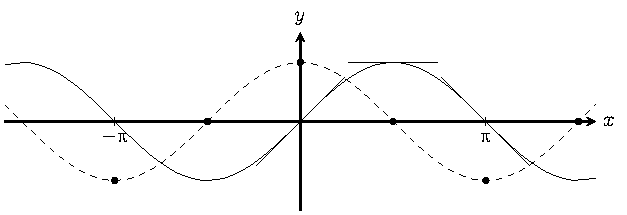
\includegraphics{basiccalculusandtrigonometry/sineandcosinerelation.pdf}
    \caption{The relation between sine and cosine}
    \label{fig:sineandcosinerelation}
\end{figure}

Illustrated in \cref{fig:sineandcosinerelation}, the slope at $x = 0$ can be approximated by a line $y = 1x + 0$: the derivative at $0$ is $1$. At $x = \flatfrac{\cpi}{2}$, the sine curve reaches its plateau: the derivative is $1$. At $x = \cpi$ it goes down by the slope $-1$, and it \emph{oscillates} like this so on and so forth. And it does this \emph{smoothly}. The function that we know of today that does this oscillatory motion smoothly is clearly a cosine. So with the graph, you can already guess that the derivative of sine must be cosine.

We shall prove this by using \cref{df:derivativenaivedefinition}: the naive definition of derivative, and the angles addition formula.
\begin{align*}
    \dv{x}\sin(x) &= \lim_{h \appr 0}\frac{\sin(x + h) - \sin(x)}{h} \\
    &= \lim_{h \appr 0}\frac{\sin(x)\cos(h) + \sin(h)\cos(x) - \sin(x)}{h} \\
    &= \lim_{h \appr 0}\frac{\sin(x)(\cos(h) - 1) + \sin(h)\cos(x)}{h}.
\end{align*}
When $h \appr 0$, $\cos(h) \appr 1$, thus $\cos(h) - 1 = 0$. And, $\sin(h) \approx h$ for very small $h$. Therefore,
\begin{align*}
    &= \lim_{h \appr 0}\frac{h\cos(x)}{h} = \cos(x).
\end{align*}

If I were to ask you again what the derivative of $\cos(x)$ is, well you can look at the graph again and instantly recognize that it's a $-\sin(x)$, and we could prove that by using the definition of derivative once again. But that would be a bit tiresome. Therefore, we can use the knowledge of cofunctions and the chain rule to help us.
\begin{equation}
    \dv{x}\cos(x) = \dv{x}\sin(\flatfrac{\cpi}{4} - x)
\end{equation}
Then, let $u = \flatfrac{\cpi}{4} - x$:
\begin{align*}
    \dv{x}\cos(x) &= \dv{x}\sin(u) \\
    &= \dv{u}\sin(u)\dv{u}{x} \\
    &= \cos(u)\dv{x}(\flatfrac{\cpi}{4} - x) \\
    &= \cos(\flatfrac{\cpi}{4} - x)(-1) = -\sin(x).
\end{align*}
Voila! The derivative of cosine is the negative of sine.

If we take the derivative of $-\sin(x)$ again, it's $-\cos(x)$\footnote{Refer back to \cref{eq:derivativesconstantmultiple}}, and of $-\cos(x)$, $\sin(x)$. Thus, the derivatives of $\sin(x)$ forms a four part loop:
\begin{gather*}
    \dv{x}\sin(x) = \cos(x), \\
    \dv{x}\cos(x) = -\sin(x), \\
    \dv{x}(-\sin(x)) = -\cos(x), \\
    \dv{x}(-\cos(x)) = \sin(x),
\end{gather*}
and the second derivative of sine is itself times a constant.

\section{Finding the power series expansion of sine and cosine}
\label{sec:taylorseriesforsineandcosine}

By using the fact that the second derivative of sine is itself times a constant, one can also extract the power series expansion of sine just like what we did in \cref{sec:afunctionthatisitsownderivative}. We begin by letting
\begin{equation}
    \sin(x) = a_0x^0 + a_1x^1 + a_2x^2 + a_3x^3 + \dots. \label{eq:taylorseriessineproof1}
\end{equation}
Then,\footnote{$0! = 1$.}
\begin{equation}
    \dv[2]{x}\sin(x) = a_2\frac{2!}{0!}x^0 + a_3\frac{3!}{1!}x^1 + a_4\frac{4!}{2!}x^2 + \dots. \label{eq:taylorseriessineproof2}
\end{equation}
The second derivative of sine must be the negative of sine, therefore
\begin{equation*}
    -a_0x^0 - a_1x^1 - a_2x^2 - a_3x^3 - \dots = a_2\frac{2!}{0!}x^0 + a_3\frac{3!}{1!}x^1 + a_4\frac{4!}{2!}x^2 + \dots
\end{equation*}
Matching the coefficient will give rise to a set of equations:
\begin{align*}
    -a_0 = \frac{2!}{0!}a_2, &\quad -a_1 = \frac{3!}{1!}a_3, \\
    -a_2 = \frac{4!}{2!}a_4, &\quad -a_3 = \frac{5!}{3!}a_5, \\
    &\vdots
\end{align*}
Or generally,
\begin{equation*}
    -a_n = \frac{(n + 2)!}{n!}a_{n + 2}.
\end{equation*}
I've intentionally write the set of equations above in two separate columns because each column is independent of one another. Here, we have to find both $a_0$ and $a_1$ that satisfies the equation.

Just like in the exponential case, when plugged $x = 0$ in, the power series is left with just $a_0$, and $\sin(0) = 0$; therefore, $a_0 = 0$. The terms following $a_0$, namely the even numbered terms, also dissapears as a consequence, leaving us with the \emph{odd} numbered terms:
\begin{equation*}
    \sin(x) = a_1x + a_3x^3 + a_5x^5 + \dots.
\end{equation*}

Now this might be a bit tricky, because there's virtually no way to get $a_1$ out by plugging anything in. Here, the small angle approximation will come in handy. Notice that we want our power series to \emph{approach} sine of $x$ with infinitely many terms. Truncating the series will obviously give us a nice approximation to sine. Here is where the small angle approximation comes in handy. Let's truncate the series at the very first term.
\begin{equation*}
    \sin(x) \approx a_1x.
\end{equation*}
\emph{This} must be an approximation for sine. Which by the small angle approximation, $\sin(x) \approx x$ where $x$ is small. Therefore, $a_1$ must be equal to one.

The rest of the equation is left for the reader as an exercise. Just take $a_1 = 1$ and go through the set of equations mentioned above. Then, you'll get that
\begin{equation}
    \sin(x) = x - \frac{1}{3!}x^3 + \frac{1}{5!}x^5 - \frac{1}{7!}x^7 + \dots, \label{eq:taylorseriessineproof3}
\end{equation}
which shall justify my statement of \cref{eq:taylorseriessine}.

Now, to find the power series of cosine, you just have to differentiate \cref{eq:taylorseriessineproof3} and get
\begin{equation*}
    \cos(x) = 1 - \frac{1}{2!}x^2 + \frac{1}{4!}x^4 - \frac{1}{6!}x^6 + \dots.
\end{equation*}
As said, truncating these polynomials will actually get you the approximation for sine and cosine. I encourage you to take out any device that can plot graphs and put the first few terms in for both sine and cosine. In case that's not available, I illustrated the power series expansion of sine up to the fifth term for the reader in \cref{fig:sineapprox}.

\begin{figure}
    \centering
    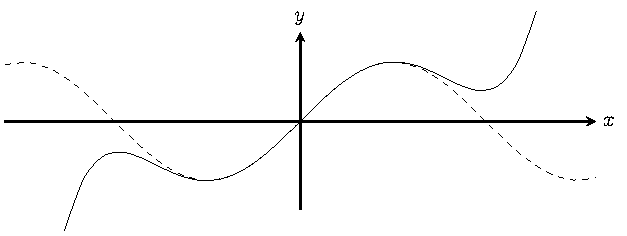
\includegraphics{basiccalculusandtrigonometry/sineapprox.pdf}
    \caption{The graph of sine (dotted) plotted with the power series expansion of sine to the fifth term.}
    \label{fig:sineapprox}
\end{figure}

\section{Derivatives of other trigonometric functions}

Note that these wouldn't be used that often until we reach \cref{sec:techniquesofintegration}

\section{Derivatives and integrals of inverse trigonometric functions}

\section{Newton's law in polar coordinates}

\section{Newton's law in cylindrical coordinates}

\section{Harmonic addition theorem}

\index{harmonic addition theorem}In this section I shall extend on the trigonometric identities a bit wit the \textbf{harmonic addition theorem} which states that it's always possible to write a sum of sinusoids with the same angular speed, $a\sin(\omega\theta) + b\cos(\omega\theta)$, as a single sinusoid $c\cos(\theta + \phi)$. I'd love if there's a clean and nice geometrical interpretation for this, but apparently there isn't.\footnote{I still have much questions with this proof here, e.g., how does this theorem goes with the phasors diagram?} So, I shall just state the theorem with the proof below.
\begin{thm}{Harmonic addition theorem}{harmonicadditionthm}
    The sum of sines and cosines with the same angular frequency $\omega$ can always be written as a sine function.
    \begin{equation*}
        a\sin(\omega \theta) + b\cos(\omega \theta) = \sgn(b)\sqrt{a^2 + b^2}\cos(\theta + \arctan(-\frac{a}{b})).
    \end{equation*}
    where the sign function $\sgn$ is defined as
    \begin{equation*}
        \sgn(x) = 
        \begin{cases*}
            -1 \quad \mathrm{if} \quad x < 0 \\
            0 \quad \mathrm{if} \quad x = 0 \\
            1 \quad \mathrm{if} \quad x > 0
        \end{cases*}
    \end{equation*}
\end{thm}

\begin{proof}
    First, notice that
    $c\cos\theta\cos\phi - c\sin\theta\sin\phi$.
\end{proof}
